\documentclass{article}                                                         
\usepackage[french]{babel}
\usepackage{geometry}
\geometry{hmargin=2.5cm,vmargin=1cm} 
\usepackage[T1]{fontenc}
\usepackage{tcolorbox,listings}
\usepackage{fullpage}
\usepackage{color}
\usepackage{graphicx}
\usepackage{float}
\usepackage[utf8]{inputenc}                                                    
\usepackage{algorithmeUTF8}
\usepackage{verbatim}
\lstset{
language=C,
literate=
{²}{{\textsuperscript{2}}}1
{⁴}{{\textsuperscript{4}}}1
{⁶}{{\textsuperscript{6}}}1
{⁸}{{\textsuperscript{8}}}1
{€}{{\euro{}}}1
{’}{'}1
{○}{{$ \circ $}}1
{●}{{$ \bullet $}}1
{é}{{\'e}}1
{è}{{\`{e}}}1
{ê}{{\^{e}}}1
{ë}{{\¨{e}}}1
{É}{{\'{E}}}1
{Ê}{{\^{E}}}1
{û}{{\^{u}}}1
{ù}{{\`{u}}}1
{â}{{\^{a}}}1
{à}{{\`{a}}}1
{á}{{\'{a}}}1
{ã}{{\~{a}}}1
{Á}{{\'{A}}}1
{Â}{{\^{A}}}1
{Ã}{{\~{A}}}1
{ç}{{\c{c}}}1
{Ç}{{\c{C}}}1
{õ}{{\~{o}}}1
{ó}{{\'{o}}}1
{ô}{{\^{o}}}1
{Õ}{{\~{O}}}1
{Ó}{{\'{O}}}1
{Ô}{{\^{O}}}1
{î}{{\^{i}}}1
{Î}{{\^{I}}}1
{í}{{\'{i}}}1
{Í}{{\~{Í}}}1,  
basicstyle=\ttfamily,
stringstyle=\ttfamily\color{green!50!black},
keywordstyle=\color{blue}\bfseries,
commentstyle=\color{red!50!black}\itshape,
showspaces=false,
showstringspaces=true,
fontadjust=true,
keepspaces=true,
flexiblecolumns=true,
frame=single,
upquote=true
}


\lstdefinestyle{frameStyle}{
basicstyle=\footnotesize,
numbers=left,
numbersep=20pt,
numberstyle=\tiny\color{black}
}

\tcbuselibrary{listings,skins,breakable}

\newtcblisting{customFrame}{
arc=0mm,
top=0mm,
bottom=0mm,
left=3mm,
right=0mm,
width=\textwidth,
listing only,
listing options={style=frameStyle},
breakable
}

\title{RAPPORT PROJET OTHELLO}                         
\author{Victorin Turnel, Paul Thulliez,Chen Yang, Ahmed Zarki, Sacha Wojciechowski}



\begin{document}
\maketitle
\newpage
\tableofcontents

\newpage

\section{Introduction}
Le jeu d'Othello, également connu sous le nom de Reversi, est un jeu de stratégie abstraite qui a été inventé au milieu du XIXe siècle. Bien que les règles du jeu soient simples, les possibilités de jeu sont infinies, ce qui en fait un défi stimulant pour les joueurs de tous niveaux.

\vspace{5mm}

C'est ainsi que dans le cadre du cours d'Algorithmique avancée, nous avons eu à réaliser le développement d'un jeu d'Othello. Nous détaillerons dans ce rapport les différentes étapes qui nous ont permis de parvenir à ce résultat. Pour cela, ce document détaillera chaque étape du cycle en V dans l'ordre. 

\vspace{5mm}

Pour continuer, nous allons détailler les principaux objectifs de ce projet. Le but de ce projet était le développement d'un jeu d'Othello ayant plusieurs fonctionnalités :
\begin{itemize}
    \item Un programme de base permettant de jouer à l'Othello
    \item Une interface Homme-Machine fonctionnelle
    \item Une intelligence artificielle
    \item Un programme permettant l'intégration d'un mode tournois
    \item Une interface Machine-Machine
    \item Une documentation
    \item Des tests unitaires
\end{itemize}

\vspace{5mm}


Enfin, rappelons les règles de l'Othello. Le jeu se joue sur un plateau de huit rangées et huit colonnes, avec deux joueurs qui s'affrontent. Les joueurs ont chacun des pions de couleur, généralement noirs et blancs. Le but du jeu est de finir avec le plus de pions de sa couleur sur le plateau.

\vspace{5mm}

Le joueur qui commence le jeu place son pion au centre du plateau, et les joueurs jouent à tour de rôle. À chaque tour, un joueur doit placer son pion sur le plateau de manière à ce qu'il encercle au moins un pion adverse, formant ainsi une chaîne de pions de sa couleur. Les pions encerclés sont alors retournés pour prendre la couleur du joueur qui vient de jouer. Si un joueur ne peut pas jouer, il doit passer son tour.

\vspace{5mm}

Le jeu se termine lorsque tous les emplacements du plateau sont occupés ou lorsque aucun joueur ne peut plus jouer. Le joueur qui a le plus de pions de sa couleur sur le plateau à la fin du jeu est déclaré vainqueur. Si le nombre de pions de chaque couleur est égal, la partie est déclarée nulle.

\newpage

\section{Analyse}

\subsection{TAD COULEUR :}
\begin{tad}
\tadNom{Couleur}
\tadDependances{Booleen}

\begin{tadOperations}{couleur}  
\tadOperation{blanc}{\tadUnParam{Couleur}}
\tadOperation{noir}{\tadUnParam{Couleur}}
\tadOperation{estBlanc}{\tadUnParam{Couleur}}{\tadUnParam{Booleen}}
\tadOperation{changerCouleur}{\tadUnParam{Couleur}}{\tadUnParam{Couleur}}
\end{tadOperations}

\begin{tadAxiomes}
\tadAxiome{estBlanc(blanc())}
\tadAxiome{non(estBlanc(noir()))}
\tadAxiome{changerCouleur(blanc())=noir()}
\end{tadAxiomes}

\end{tad}

\subsection{TAD PION :}
\begin{tad}
\tadNom{Pion}
\tadDependances{Couleur}

\begin{tadOperations}{creerPion}  
\tadOperation{creerPion}{\tadUnParam{Couleur}}{\tadUnParam{Pion}}
\tadOperation{obtenirCouleurSuperieure}{\tadUnParam{Pion}}{\tadUnParam{Couleur}}
\tadOperation{retourner}{\tadUnParam{Pion}}{\tadUnParam{Pion}}
\end{tadOperations}

\begin{tadAxiomes}
\tadAxiome{obtenirCouleurSuperieure(retournerPion(creerPion(col) != col}
\end{tadAxiomes}

\end{tad}


\subsection{TAD POSITION :}
\begin{tad}
	\tadNom{Position}
	\tadDependances{1..8}
	\begin{tadOperations}{Position}
		\tadOperation{position}{\tadDeuxParams{1..8}{1..8}}{Position}
		\tadOperation{obtenirX}{Position}{1..8}
		\tadOperation{obtenirY}{Position}{1..8}
	\end{tadOperations}
	\begin{tadAxiomes}
		\tadAxiome{obtenirX(Position(x,y))=x}
		\tadAxiome{obtenirY(Position(x,y))=y}
	\end{tadAxiomes}
	
	
\end{tad}


\subsection{TAD COUP :}
\begin{tad}
	\tadNom{Coup}
	\tadDependances{Pion,Position}
	\begin{tadOperations}{Coup}
		\tadOperation{coup}{\tadDeuxParams{Pion}{Position}}{\tadUnParam{Coup}}
		\tadOperationAvecPreconditions{obtenirPionCoup}{\tadUnParam {Coup}}{\tadUnParam{Pion}}
		\tadOperationAvecPreconditions{obtenirPositionCoup}{\tadUnParam{Coup}}{\tadUnParam{Position}}
        \end{tadOperations}
              
	\begin{tadAxiomes}
          \tadAxiome{obtenirPionCoup(coup(pion,pos))=pion}
          \tadAxiome{obtenirPositionCoup(coup(pion,pos))=pos}
	\end{tadAxiomes}


\end{tad}


\subsection{TAD COUPS :}
\begin{tad}
	\tadNom{Coups}
	\tadDependances{Coup, NNN, Naturel}
	\begin{tadOperations}{Coups}
		\tadOperation{Coups}{}{\tadUnParam{Coups}}
		\tadOperation{nbCoups}{Coups}{Naturel}
		\tadOperation{ajouterCoups}{\tadDeuxParams{Coups}{Coup}}{Coups}
		\tadOperationAvecPreconditions{iemeCoup}{\tadDeuxParams{Coups}{NNN}}{Coup}
	\end{tadOperations}
	\begin{tadPreconditions}{Coups}
		\tadPrecondition{iemeCoups(coups,position)}{position $\leq$ nbCoups(coups)}
	\end{tadPreconditions}
	\begin{tadAxiomes}
		\tadAxiome{Coups()}
		\tadAxiome{nbCoups(Coups())=0}
		\tadAxiome{nbCoups(ajouterCoups(coups,coup)) = nbCoups(coups) +1}
		\tadAxiome{iemeCoup(ajouterCoups(coups,coup),nbCoups(coups)+1 ) = coup}
	\end{tadAxiomes}


\end{tad}
        


\subsection{TAD PLATEAU :}

\begin{tad}


\tadNom{Plateau}
\tadDependances{Pion, Position, \booleen}

\begin{tadOperations}{retournerPion}
	\tadOperation{plateau}{}{\tadUnParam{Plateau}}
	\tadOperationAvecPreconditions{poserPion}{\tadTroisParams{Position}{Pion}{Plateau}}{\tadUnParam{Plateau}}
	\tadOperationAvecPreconditions{obtenirPion}{\tadDeuxParams{Position}{Plateau}}{\tadUnParam{Pion}}
	\tadOperation{caseVide}{\tadDeuxParams{Position}{Plateau}}{\tadUnParam{\booleen}}
	\tadOperationAvecPreconditions{retournerPion}{\tadDeuxParams{Position}{Plateau}}{\tadUnParam{Plateau}}
	\tadOperationAvecPreconditions{enleverPion}{\tadDeuxParams{Position}{Plateau}}{\tadUnParam{Plateau}}
\end{tadOperations}

\begin{tadPreconditions}{poserPion(pos,pion,pl)}
	\tadPrecondition{obtenirPion(pos,pl)}{non (caseVide(pos,pl))}	
	\tadPrecondition{retournerPion(pos,pl)}{non (caseVide(pos,pl))}
	\tadPrecondition{poserPion(pos,pion,pl)}{caseVide(pos,pl)}
	\tadPrecondition{enleverPion(pos,pl)}{non (caseVide(pos,pl))}
\end{tadPreconditions}

\begin{tadAxiomes}
	\tadAxiome{caseVide(pos,plateau())}
	\tadAxiome{obtenirPion(pos,poserPion(pos,pion,plateau()))= pion}
	\tadAxiome{caseVide(pos,enleverPion(pos,plateau()))}
	\tadAxiome{non caseVide(pos,poserPion(pos,pion,plateau()))}
	\tadAxiome{retournerPion(pos,retournerPion(pos,pl))=pl}	
\end{tadAxiomes}
\end{tad}

\documentclass{article}
\usepackage[french]{babel}
\usepackage[T1]{fontenc}
\usepackage[utf8x]{inputenc}
\usepackage{algorithmeUTF8}



\subsection{Analyse descendante de la fonction faireUnePartie}

\begin{figure}[H]
    \rotatebox{90}{\includegraphics[width=23cm,height=15cm]{analyse/ADFaireUnePartie.pdf}}
    \caption{Analyse descendante de faireUnePartie}
    \label{un-identifiant1}
\end{figure}

\subsection{Analyse descendante de la fonction obtenirCoup}

\begin{figure}[H]                                                                                                                                                                                             
    \rotatebox{90}{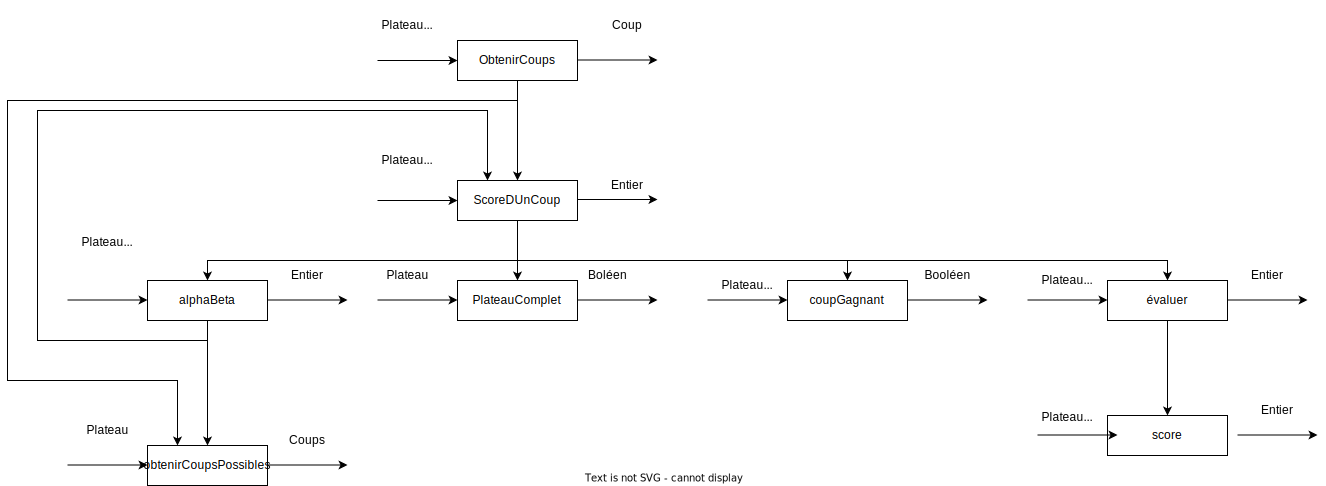
\includegraphics[width=23cm,height=10cm]{analyse/ADobtenirCoup.pdf}}                                                                                                               
    \caption{Analyse descendante de obtenirCoup}                                                                                                                          
    \label{un-identifiant2}                                                                                                                                                                                 
\end{figure} 

\newpage      

\section{Conception préliminaire}

\subsection{TAD : Couleur}
\begin{algorithme}
  \signaturefonction{blanc}{}{Couleur}
  
  \vspace*{5mm}
  
  \signaturefonction{noir}{}{Couleur}

  \vspace*{5mm}
  
  \signaturefonction{estBlanc}{couleur : Couleur}{\booleen}

  \vspace*{5mm}
  
  \signaturefonction{changerCouleur}{couleur: Couleur}{Couleur}
\end{algorithme}


\subsection{TAD : Pion}
\begin{algorithme}
  \signaturefonction{creerPion}{couleur : Couleur}{Pion}
  \signaturefonction{obtenirCouleurSuperieure}{pion : Pion}{Couleur}
  \signatureprocedure{retournerPion}{\paramEntree{pion : Pion},\paramSortie{Pion}}
\end{algorithme}
  


\subsection{TAD : Position}
\input{cp/position/CPTADposition}

\subsection{TAD : Coup}
\begin{algorithme}
\signaturefonction{coupCoup}{pion:Pion,pos:Position}{Coup}
\signaturefonction{coupObtenirPionCoup}{coup:Coup}{Pion}
\signaturefonction{coupObtenirPositionCoup}{coup:Coup}{Position}
\end{algorithme}


\subsection{TAD : Plateau}
\begin{algorithme}
  \signaturefonction{plateau}{}{Plateau}
  \signatureprocedure{poserPion}{\paramEntreeSortie{plateau : Plateau} , \paramEntree{pos : Position , pion: Pion}}

  \vspace*{5mm}
  
  \preconditions{estCaseVide(plateau , pos)}

  \vspace*{5mm}
  
  \signaturefonction{obtenirPion}{plateau : Plateau , pos : Position}{Pion}

  \vspace*{5mm}

  \preconditions{non (estCaseVide(plateau , pos)}

  \vspace*{5mm}
  
  \signaturefonction{estCaseVide}{plateau : Plateau , pos : Position}{\booleen}

  \vspace*{5mm}
  
  \signatureprocedure{retournerPion}{\paramEntreeSortie{plateau : Plateau} , \paramEntree{pos : Position}}

  \vspace*{5mm}
  
  \preconditions{non(estCaseVide(plateau , pos)}

  \vspace*{5mm}
  
  \signatureprocedure{enleverPion}{\paramEntreeSortie{plateau : Plateau},\paramEntree{pos : Position}}

  \vspace*{5mm}
  
  \preconditions{non(estCaseVide(plateau , pos)}
\end{algorithme}


\subsection{faireUnePartie}
\begin{algorithme}
  \type{EtatPartie}{[TERMINE,ENCOURS]}
\end{algorithme}

\begin{algorithme}
\signatureprocedure{afficherPlateau}{\paramSortie{p:Plateau}}
	\type{AffichagePlateau}{afficherPlateau}
\end{algorithme}

\begin{algorithme}
  \signaturefonction{obtenirCoupEnFctDuJoueur}{p : Plateau, joueur : Couleur}{Coup}
	\type{ObtenirCoupEnFctDuJoueur}{obtenirCoupEnFctDuJoueur}
\end{algorithme}

\begin{algorithme}
	\signaturefonction{faireUnePartie}{obtenirCoupJoueurNoir,obtenirCoupJoueurBlanc : ObtenirCoupEnFctDuJoueur, plateauAAfficher : AffichagePlateau}{Couleur}
	\signaturefonction{initialiserPlateau}{}{Plateau}
	\signaturefonction{etatPartie}{plateau:Plateau}{gagnant : Couleur,etatPartie : EtatPartie}
	\signaturefonction{plateauTotalementRempli}{plateau:Plateau}{\booleen}
	\signaturefonction{plateauBloque}{plateau:Plateau}{\booleen}
	\signaturefonction{evaluer}{p:Plateau,couleurAEvaluer:Couleur}{\entier}
	\signatureprocedure{jouer}{\paramEntreeSortie {plateau : Plateau} , \paramEntree{coup : Coup}}
	\signaturefonction{coupLegal}{plateau:Plateau , coup : Coup}{\booleen}
	\signatureprocedure{retournerPionsEmprisonnes}{\paramEntreeSortie {plateau : Plateau} , \paramEntree{coup : Coup, coups : Coups }}
	\signaturefonction{adversairesAdjacents}{plateau:Plateau , coup : Coup}{Coups}
	\signaturefonction{pionMemeCouleur}{plateau:Plateau , coup : Coup, coups : Coups}{Coups}
	\signaturefonction{coupEnFctJoueur}{couleurJoueur : Couleur,obtenirCoupJoueurNoir,obtenirCoupJoueurBlanc : ObtenirCoupEnFctDuJoueur}{Coup}
\end{algorithme}



\subsection{obtenirCoup}

\begin{algorithme}
	\signaturefonction
	{obtenirCoup}
	{unPlateau : \textbf{Plateau}, joueur : \textbf{Couleur}, profondeur : \naturel}
	{\textbf{Coup}}
	\preconditions{non plateauComplet(unPlateau)}
	
	\vspace{5mm}
	
	
	\signaturefonction
	{scoreDUnCoup}
	{unPlateau : \textbf{Plateau}, joueurRef, joueurCourant : \textbf{Couleur}, unCoup : \textbf{Coup}, profondeur : \naturel, alpha, beta : \entier}
	{\entier}
	
	\vspace{5mm}
	
	
	\signaturefonction
	{alphaBeta}
	{unPlateau : \textbf{Plateau}, joueurRef, joueurCourant : \textbf{Couleur}, profondeur : \naturel, alpha, beta : \entier}
	{\entier}
	
	\vspace{5mm}
	
	
	\signaturefonction
	{evaluer}
	{unPlateau : \textbf{Plateau}, joueurRef : \textbf{Couleur}}
	{\entier}
	
	\vspace{5mm}
	
	
	\signaturefonction
	{score}
	{unPlateau : \textbf{Plateau}, joueur : \textbf{Couleur}}
	{\entier}
	
	\vspace{5mm}
	
	
	\signaturefonction
	{obtenirCoupsPossibles}
	{unPlateau : \textbf{Plateau}, joueurRef : \textbf{Couleur}}
	{\textbf{Coups}}
	
	\vspace{5mm}
	
	\signaturefonction
	{compteurCouleur}
	{plateau : \textbf{Plateau}, couleur : \textbf{Couleur}}
	{\naturel}
	
	
	\vspace{5mm}
	
	\signaturefonction
	{plateauBloquePourUneCouleur}
	{unPlateau : \textbf{Plateau}, laCouleur : \textbf{Couleur}}
	{\booleen}
	
	\vspace{5mm}
	
	\signaturefonction
	{plateauBloque}
	{unPlateau : \textbf{Plateau}}
	{\booleen}
	
	
\end{algorithme}



\newpage

\section{Conception détaillée}
\subsection{Conception détaillée des fonctions des TAD :}

\subsubsection{TAD COULEUR :}
\begin{algorithme}
  \type{Couleur}{\{Blanc,Noir\}}
\end{algorithme}

\vspace*{1cm}


\begin{algorithme}
  \small
  \fonction{couleurBlanc}{}{Couleur}
  {}
    {\retourner{Blanc}}

\end{algorithme}


\vspace*{1cm}

\begin{algorithme}
  \small
  \fonction{couleurNoir}{}{Couleur}
  {}
   {\retourner{Noir}}

\end{algorithme}

\vspace*{1cm}

\begin{algorithme}
  \small
  \fonction{couleurEstBlanc}{couleur:Couleur}{\booleen}
  {}
  {\retourner{couleur=Blanc}}

\end{algorithme}

\vspace*{1cm}

\begin{algorithme}
  \small
  \fonction{couleurChangerCouleur}{couleur:Couleur}{Couleur}
  {}
  {\sialorssinon{couleurEstBlanc(couleur)}{\affecter{couleur}{Noir} \retourner{couleur}}{\affecter{couleur}{Blanc} \retourner{couleur}}}

\end{algorithme}


\subsubsection{TAD PION :}
\begin{algorithme}

  \begin{enregistrement}{Pion}
    \champEnregistrement{couleur : Couleur}
  \end{enregistrement}

  \vspace*{5mm} 
  
  \fonction
      {creerPion}
      {couleur : Couleur}
      {Pion}
      {pion : Pion}
      {{\affecter{pion.Couleur}{couleur}}

       {\retourner {pion}}}

  \vspace*{5mm} 
      
  \fonction
      {obtenirCouleurSuperieure}
      {pion : Pion}
      {Couleur}
      {couleur : Couleur}
      {\retourner {pion.Couleur}}

  \vspace*{5mm} 
      
  \procedure
      {retournerPion}
      {\paramEntreeSortie{pion : Pion}}
      {}
      {changeCouleur(pion.Couleur)}

\end{algorithme}


\subsubsection{TAD POSITION :}
\begin{algorithme}
	
	\begin{enregistrement}{Pion}
		\champEnregistrement{x}{\textbf{1..LARGEUR\_PLATEAU}}
		\champEnregistrement{y}{\textbf{1..HAUTEUR\_PLATEAU}}
	\end{enregistrement}
	
	\vspace*{5mm} 
	
	\fonction
	{position}
	{largeur : \textbf{1..LARGEUR\_PLATEAU}, hauteur : \textbf{1..HAUTEUR\_PLATEAU}}
	{\textbf{Position}}
	{resultat : Position}
	{\affecter{resultat.x}{largeur}
		\affecter{resultat.y}{hauteur}
		\retourner {resultat}}
	
	\vspace*{5mm} 
	
	\fonction
	{obtenirX}
	{unePosition : \textbf{Position}}
	{\textbf{1..LARGEUR\_PLATEAU}}
	{}
	{\retourner {pion.x}}
	
	\vspace*{5mm} 
	
	\fonction
	{obtenirY}
	{unePosition : \textbf{Position}}
	{\textbf{1..HAUTEUR\_PLATEAU}}
	{}
	{\retourner {pion.y}}
	
	
\end{algorithme}

\subsubsection{TAD COUP :}
\begin{algorithme}
  \begin{enregistrement}{Coup}
    \champEnregistrement{pion}{Pion}
    \champEnregistrement{position}{Position}
  \end{enregistrement}
\end{algorithme}

\begin{algorithme}
  \small
  \fonction{coupCoup}{pion:Pion,pos:Position}{Coup}
           {}
           {\affecter{coup.position}{pos}
            \affecter{coup.pion}{pion}
            \retourner{coup}
           }
 
\end{algorithme}

\begin{algorithme}
  \small
  \fonction{coupObtenirPionCoup}{coup:Coup}{Pion}
           {}
           {\retourner{coup.pion} 
           }
  
\end{algorithme}

\begin{algorithme}
  \small
  \fonction{coupObtenirPositionCoup}{coup:Coup}{Position}
           {}
           {\retourner{coup.position}
           }
  
\end{algorithme}


\subsubsection{TAD COUPS :}
\begin{algorithme}
  
  \begin{enregistrement}{Coups}
    \champEnregistrement{lesCoups}{\textbf{Tableau[1..LARGEUR\_PLATEAU*HAUTEUR\_PLATEAU] de Coup}}
    \champEnregistrement{nbTotalCoups}{\naturel}
  \end{enregistrement}
\end{algorithme}

\vspace*{5mm}

\begin{algorithme}
  \small
  \fonction
      {coups}
      {}
      {\textbf{Coups}}
      {coups : \textbf{Coups}}
      {\affecter{coups.nbTotalCoups}{0}
	\retourner {coups}}
\end{algorithme}

\vspace*{5mm} 

\begin{algorithme}
  \small
  \fonction
      {nbCoups}
      {coups : \textbf{Coups}}
      {\naturel}
      {}
      {\retourner {coups.nbTotalCoups}}
\end{algorithme}

\vspace*{5mm} 

\begin{algorithme}
  \small
  \procedure
      {ajouterCoups}
      {\paramEntreeSortie{coups : \textbf{Coups}},\paramEntree{coup : \textbf{Coup}}}
      {}
      {\affecter{coups.nbTotalCoups}{coups.nbTotalCoups+1}
	\affecter{coups.lesCoups[coups.nbTotalCoups]}{coup}}
\end{algorithme}

\vspace*{5mm} 

\begin{algorithme}
  \small
  \fonction
      {iemeCoup}
      {coups : \textbf{Coups}, place : \textbf{NNN} }
      {\textbf{Coup}
	\preconditions{place $\leq$ nbCoups(coups)}}
      {}
      {\retourner {coups.lesCoups[place]}}
      
\end{algorithme}


\subsubsection{TAD PLATEAU :}
\begin{algorithme}
  \begin{enregistrement}{Case}
    \champEnregistrement{estVide}{\booleen}
    \champEnregistrement{pion}{Pion}
  \end{enregistrement}
  
  \vspace*{5mm}
  
\end{algorithme}

\vspace*{5mm}

\begin{algorithme}
  \type{\textbf{Plateau}}{Tableau[8][8] de \textbf{Case}}
\end{algorithme}

\vspace*{5mm}

\begin{algorithme}
  \small
  \fonction
      {plateau}
      {}
      {\textbf{Plateau}}
      {plateau : \textbf{Plateau} , i,j:\naturel}
      {
        \pour{i}{1}{8}{}
	     {
               \pour{j}{1}{8}{}
	            {
                      \affecter{plateau[i][j].estVide}{Vrai}
                    }
	     }
	     \retourner {plateau}
      }
\end{algorithme}

\vspace*{5mm}

\begin{algorithme}
  \small
  \procedureAvecPreconditions
      {poserPion}
      {\paramEntreeSortie {plateau : \textbf{Plateau}} , \paramEntree {pos : \textbf{Position} , pion : \textbf{Pion}}}
      {estCaseVide(pos,plateau)}
      {x,y : \textbf{1...8}}
      {\affecter{x}{obtenirX(pos)}
    	\affecter{y}{obtenirY(pos)}
    	\affecter{plateau[x][y].pion}{pion}
    	\affecter{plateau[x][y].estVide}{Faux}
      }
\end{algorithme}

\vspace*{5mm}

\begin{algorithme}
  \small
  \fonctionAvecPreconditions
      {obtenirPion}
      {pos : \textbf{Position} , plateau : \textbf{Plateau}}
      {\textbf{Pion}}
      {non estCaseVide(plateau,pos)}
      {x,y : \textbf{1...8}}
      {
        \affecter{x}{obtenirX(pos)}
    	\affecter{y}{obtenirY(pos)}
    	\retourner {plateau[x][y].pion}
      }
\end{algorithme}

\vspace*{5mm}

\begin{algorithme}
  \small
  \procedureAvecPreconditions
      {retournerPion}
      {\paramEntreeSortie{plateau : \textbf{Plateau}} , \paramEntree{pos : \textbf{Position}}}
      {non estCaseVide(plateau,pos)}
      {pion : \textbf{Pion}}
      {
    	\affecter{pion}{obtenirPion(pos , plateau)}
    	\instruction{Pion.retournerPion(pion)}
    	\instruction{enleverPion(plateau,pos)}
    	\instruction{poserPion(plateau,pos,pion)}
      }
\end{algorithme}

\vspace*{5mm}

\begin{algorithme}
  \small
  \fonction
      {estCaseVide}{plateau :\textbf{Plateau} , pos : \textbf{Position}}
      {\booleen}
      {x,y : \textbf{1...8}}
      {
        \affecter{x}{obtenirX(pos)}
    	\affecter{y}{obtenirY(pos)}
    	\retourner {plateau[x][y].estVide}
      }
\end{algorithme}

\vspace*{5mm}

\begin{algorithme}
  \small
  \procedureAvecPreconditions
      {enleverPion}
      {\paramEntreeSortie{plateau : \textbf{Plateau}} , \paramEntree{pos : \textbf{Position}}}
      {non estCaseVide(plateau,pos)}
      {x,y : \textbf{1...8}}
      {
        \affecter{x}{obtenirX(pos)}
    	\affecter{y}{obtenirY(pos)}
        \affecter{plateau[x][y].estVide}{Vrai}
      }
      
      
\end{algorithme}



\subsection{Conception détaillée des fonctions d'obtenirCoup}
\begin{algorithme}
	\small
	\fonction
	{obtenirCoup}
	{unPlateau : \textbf{Plateau}, joueur : \textbf{Pion}, profondeur : \naturel}
	{\textbf{Coup}}
	{resultat : \textbf{Coup}, cps : \textbf{Coups}, score, meilleurScore : \entier, i : \naturel}
	{\affecter{cps}{obtenirCoupsPossibles(unPlateau)}
		\affecter{resultat}{ieme(cps,1)}
		\affecter{meilleurScore}{scoreDUnCoup(unPlateau,resultat,joueur,joueur,profondeur)}
		\pour{i}{2}{nb(cps)}{}
		{
			\affecter{score}{scoreDUnCoup(unPlateau,ieme(cps,i),joueur,joueur,profondeur)}
			\sialors{score $>$ meilleurScore}
			{
				\affecter{resultat}{ieme(cps,i)}
				\affecter{meilleurScore}{score}
			}
		}
		\retourner{resultat}
	}
	
	\vspace*{1cm}
	
	\small
	\fonction
	{obtenirCoupsPossibles}
	{unPlateau : \textbf{Plateau}, joueurRef : \textbf{Pion}}
	{\textbf{Coups}}
	{resultat : \textbf{Coups}, i : \naturel, temp : \textbf{Position}}
	{	\affecter{resultat}{coups()}
		\pour{i}{1}{HAUTEUR\_PLATEAU}{}
		{
			\pour{j}{1}{LARGEUR\_PLATEAU}{}
			{
				\affecter{coupTemp}{coup(joueurRef,position(j,i))}
				\sialors{coupLegal(unPlateau,coupTemp)}
				{
					\instruction{ajouterCoups(resultat,temp)}
				}
			}
			
		}
		\retourner{resultat}
	}
	
	\vspace*{1cm}
	
	\small
	\fonction
	{evaluer}
	{unPlateau : \textbf{Plateau}, joueurRef : \textbf{Pion}}
	{\entier}
	{}
	{	\retourner{\instruction{score(unPlateau,joueurRef)-score(unPlateau,joueurRef)}}
	}
	
	\vspace*{1cm}
	
	\small
	\fonction
	{scoreDUnCoup}
	{unPlateau : \textbf{Plateau}, joueurRef, joueurCourant : \textbf{Couleur}, unCoup : \textbf{Coup}, profondeur : \naturel, alpha, beta : \entier}
	{\entier}
	{}
	{	\instruction{jouer(unPlateau,unCoup)}
		\sialorssinon{plateauTotalementRempli(unPlateau) ou coupGagnant(unPlateau,unCoup) ou (plateauBloque(unPlateau,joueurCourant) et plateauBloque(unPlateau,autreCouleur(joueurCourant))) ou profondeur = 0}
		{
			\retourner{evaluer(unPlateau,joueurRef)}
		}
		{
			\sialors{non(plateauBloque(unPlateau,autreCouleur(joueurCourant)))}
			{
				\affecter{joueurCourant}{autreJoueur(joueurCourant)}
			}
			
			\retourner{alphaBeta(unPlateau,joueurRef,joueurCourant,profondeur-1,alpha,beta)}
		}
		
	}
	
	\vspace*{1cm}
	
	\small
	\fonction
	{alphaBeta}
	{unPlateau : \textbf{Plateau}, joueurRef, joueurCourant : \textbf{Couleur}, profondeur : \naturel, alpha, beta : \entier}
	{\entier}
	{coupsPossibles : \textbf{Coups}, resultat, score : \entier, i : \naturel}
	{	\affecter{coupsPossibles}{obtenirCoupsPossibles(unPlateau,joueurCourant)}
		\affecter{resultat}{scoreDUnCoup(unPlateau,joueurRef,joueurCourant,iemeCoup(coupsPossibles,1), profondeur,alpha,beta)}
		\pour{i}{2}{nbCoups(coupsPossibles)}{}
		{
			\affecter{score}{scoreDUnCoup(unPlateau,joueurRef,joueurCourant,iemeCoup(coupsPossibles,i), profondeur,alpha,beta)}
			\sialorssinon{joueurCourant = joueurRef}
			{
				\affecter{resultat}{max(resultat,score)}
				\sialors{resultat $\leq$ alpha}
				{
					\retourner{resultat}
				}
				\affecter{beta}{min(beta,resultat)}
			}
			{
				\affecter{resultat}{min(resultat,score)}
				\sialors{beta $\leq$ resultat}
				{
					\retourner{resultat}
				}
				\affecter{alpha}{max(alpha,resultat)}
			}
		}
		
	}
	
	\vspace*{1cm}
	
	\small
	\fonction
	{compteurCouleur}
	{plateau : Plateau, couleur : Couleur}
	{Naturel}
	{compteur : Naturel, i,j : 1..8, pos : Position}
	{\affecter{res}{0}
		\pour{i}{1}{8}{}
		{\pour{j}{1}{8}{}
			{\affecter{pos}{position(i,j)}
				\sialors{non(estCaseVide(pos,plateau)) et (obtenirCouleurSuperieur(obtenirPion(pos,plateau)) = couleur)}
				{\affecter{compteur}{compteur+1}}
			}
		}
		\retourner{compteur}
	}
	
	\vspace*{1cm}

        \small
        \fonction                                                                                                                                                                                        
            {coupGagnant}                                                                                                                                                                               
            {unPlateau : Plateau, unCoup : Coup}     
            {\booleen}
            {plateauTemp : Plateau,pion : Pion, pos : Position, couleur, couleurInverse : Couleur, compteurJoueurCourant,compteurJoueurAdv : Entiers}
            { \affecter{pion}{coupObtenirPionCoup(unCoup)}
              \affecter{couleur}{obtenirCouleurSuperieur(pion)}
              \affecter{plateauTemp}{unPlateau}        
              \affecter{couleurInverse}{couleurChangerCouleur(couleur)}
              \instruction{jouer(plateauTemp,unCoup)}                    
              \affecter{compteurJoueurCourant}{compteurCouleur(plateauTemp,couleur)}
              \affecter{compteurJoueurAdv}{compteurCouleur(plateauTemp,couleurInverse)}
              \retourner{(compteurJoueurAdv = 0) ou (compteurJoueurCourant = 0)}                                                                                                                        
           }                               
	
	\vspace*{1cm}
	
	\small
	\fonction
	{plateauBloque}
	{unPlateau : Plateau}
	{\booleen}
	{lesCoupsNoirs, lesCoupsBlancs : Coups}
	{\affecter{lesCoupsBlancs}{obtenirCoupsPossibles(unPlateau,couleurBlanc())}
		\affecter{lesCoupsNoirs}{obtenirCoupsPossibles(unPlateau,couleurNoir())}
		\sialorssinon{lesCoupsNoirs.nbCoups = 0 et lesCoupsBlancs.nbCoups = 0}
		{\retourner{VRAI}}
		{\retourner{FAUX}}
	}
	
	\vspace*{1cm}
	
	\small
	\fonction
	{score}
	{unPlateau : \textbf{Plateau}, joueur : \textbf{Couleur}}
	{\entier}
	{}
	{	\retourner{compteurCouleur(unPlateau, joueur)}
	}
	
	
\end{algorithme}


\subsection{Conception détaillée des fonctions de faireUnePartie}
\begin{algorithme}
  \type{EtatPartie}{[TERMINE,ENCOURS]}
\end{algorithme}


\begin{algorithme}
  \signaturefonction{obtenirCoupEnFctDuJoueur}{p : Plateau, joueur : Couleur}{Coup}
	\type{ObtenirCoupEnFctDuJoueur}{obtenirCoupEnFctDuJoueur}
\end{algorithme}

\begin{algorithme}
  \small
  \procedure
  {faireUnePartie}
  {\paramEntree{obtenirCoupBlanc,obtenirCoupJoueurNoir : ObtenirCoupEnFctDuJoueur}, \paramEntree{sortie : afficherPlateau} \paramEntreeSortie{couleurGagnant: Couleur}, \paramEntreeSortie{etat : EtatPartie}}
  {
  plateau: Plateau;
  joueurCourant: Pion;
  prochainCoup: Coup;
  partieEnCours: etat;
  start,end: time_t;
  }
  { 
    \affecter{joueurCourant}{creerPion(BLANC)}
    \affecter{plateau}{initialiserPlateau()}
    \repeter{
      \affecter{start}{time(NULL)}
      \repeter{
        \affecter{prochainCoup}{coupEnFctJoueur(obtenirCoupBlanc, obtenirCoupNoir, obtenirCouleurSuperieure(joueurCourant), plateau)}
      }
      {non(coupLegal(plateau,prochainCoup))}
      jouer(plateau, prochainCoup)\\
      \affecter{end}{time(NULL)}
      \sialors{difftime(start, end)$<$1}
      {
        sleep(1)
      }
      afficherPlateau(plateau,prochainCoup,1)\\
      retournerPion(joueurCourant)\\
      \sialors{plateauBloquePourUneCouleur(plateau,obtenirCouleurSuperieure(joueurCourant))}
      {
        retournerPion(joueurCourant)
        afficherPlateau(plateau,prochainCoup,0)
      }
      etatPartie(plateau, couleurGagnant, etat)
    }{etat=partieEnCours}
  }
\end{algorithme}



\newpage

\section{Code}

\subsection{Header}

\subsubsection{Couleur}
\lstinputlisting[language = C]{../programme/include/TADcouleur.h}

\subsubsection{Pion}
\lstinputlisting[language = C]{../programme/include/TADpion.h}

\subsubsection{Position}
\lstinputlisting[language = C]{../programme/include/TADposition.h}

\subsubsection{Coup}
\lstinputlisting[language = C]{../programme/include/TADcoup.h}

\subsubsection{Coups}
\lstinputlisting[language = C]{../programme/include/TADcoups.h}

\subsubsection{Plateau}
\lstinputlisting[language = C]{../programme/include/TADplateau.h}

\subsubsection{faireUnePartie}
\lstinputlisting[language = C]{../programme/include/faireUnePartie.h}

\subsubsection{obtenirCoup}
\lstinputlisting[language = C]{../programme/include/obtenirCoup.h}

\subsubsection{obtenirCoupPrive}
\lstinputlisting[language = C]{../programme/include/obtenirCoupPrive.h}

\subsection{Interface Homme-Machine}
\lstinputlisting[language = C]{../programme/include/IHM.h}

\subsection{Interface Machine-Broker}
\lstinputlisting[language = C]{../programme/include/IMB.h}

\subsection{Source}

\subsubsection{Couleur}
\lstinputlisting[language = C]{../programme/src/TADcouleur.c}

\subsubsection{Pion}
\lstinputlisting[language = C]{../programme/src/TADpion.c}

\subsubsection{Position}
\lstinputlisting[language = C]{../programme/src/TADposition.c}

\subsubsection{Coup}
\lstinputlisting[language = C]{../programme/src/TADcoup.c}

\subsubsection{Coups}
\lstinputlisting[language = C]{../programme/src/TADcoups.c}

\subsubsection{Plateau}
\lstinputlisting[language = C]{../programme/src/TADplateau.c}

\subsubsection{faireUnePartie}
\lstinputlisting[language = C]{../programme/src/faireUnePartie.c}

\subsubsection{obtenirCoup}
\lstinputlisting[language = C]{../programme/src/obtenirCoup.c}

\subsection{Interface Homme-Machine}                                                                                                                                                                      
\lstinputlisting[language = C]{../programme/src/IHM.c}                                                                                                                                               
                                                                                                                                                                                                         
\subsection{Interface Machine-Broker}                                                                                                                                                                    
\lstinputlisting[language = C]{../programme/src/IMB.c}                                                                                                                                                
                                                            
\newpage

\section{Conclusion}
\subsection{Rétrospective}

En conclusion, notre projet de programmation d'un jeu d'Othello en C a été un défi intéressant qui nous a permis de mettre en pratique nos compétences en programmation C et en intelligence artificielle. Nous avons développé une intelligence artificielle qui utilise l'algorithme min-max avec élagage alpha-bêta, capable de jouer de manière compétitive au jeu en utilisant des techniques de recherche en profondeur et d'évaluation de l'état du jeu.

\vspace{5mm}

Nous avons rencontré plusieurs défis au cours de ce projet :
\begin{itemize}
\item Avoir une bonne communication dans le groupe
\item Utiliser correctement Git
\item Utiliser un langage de programmation qui nous était inconnu
\item Utiliser une méthode de développement rigoureuse
\item Savoir faire preuve d'autonomie et de gestion de groupe
\item Respecter les délais
\end{itemize}

\vspace{5mm}

Nous avons réussi à les surmonter grâce à notre persévérance et à notre capacité à trouver des solutions créatives. Les résultats de notre travail ont été concluants, et nous avons réussi à atteindre notre objectif avec un programme parfaitement fonctionnel.

\vspace{5mm}

En fin de compte, ce projet a été une expérience très enrichissante qui nous a permis de nous améliorer en tant que programmeurs et de découvrir de nouvelles techniques de programmation. De plus, nous avons appris à utiliser de nouveaux outils qui nous seront très utiles dans le futur.

\subsection{Repartition des tâches}
\begin{tabular}{|l|c|c|c|c|c|}
  \hline
  Tâches & Ahmed Zarki & Victorin Turnel & Chen Yang & Paul Thulliez & Sacha Wojciechowski \\
  \hline
  Analyse \\
  \hline
  faireUnePartie & & & X & & \\
  obtenirCoup & & X & & & \\
  TAD Couleur  & & & X & X & \\
  TAD Pion & & & & & X \\
  TAD Position & & X & & & \\
  TAD Coup & & & & X & \\
  TAD Coups & & X  & & &  \\
  TAD Plateau & X & & & & \\
  \hline
  Conception préliminaire \\
  \hline
  CP TAD Couleur & & & X & X & \\
  CP TAD Pion & & & & & X \\
  CP TAD Postion & & X & & & \\
  CP TAD Coup & & & & X & \\              
  CP TAD Coups & & X & & & \\             
  CP TAD Plateau & X & & & & \\
  \hline
  Conception détaillé \\
  \hline
  CD TAD Couleur & & & X & X & \\                                                                                                                                                                       
  CD TAD Pion & & & & & X \\                                                                                   
  CD TAD Postion & & X & & &  \\                                                                                                                                                                         
  CD TAD Coup & & & & X & \\                                                                                                                                                                             
  CD TAD Coups & & X & & & \\                                                                                                                                                                            
  CD TAD Plateau & X & & & & \\                              
  Mise en page rapport & X & & & & X \\      
  Makefile rapport & & & & & X \\
  \hline
  Developpement \\
  \hline
  TAD Couleur & X & & & & \\                                                                                                                                                                       
  TAD Pion & & & X & & \\                                                                                                                                                                              
  TAD Postion & & & & X &  \\                                                                                                                                                                          
  TAD Coup & & X & &  & \\                                                                                                                                                                              
  TAD Coups & & & & X & \\                                                                                                                                                                             
  TAD Plateau & & & & & X \\                                                                                                                                                                      
  obtenirCoup & & X & & & X \\
  compteurCouleur & & & & & X \\
  score & & & & & X \\
  evaluer & & & & & X \\
  plateauBloque & & & & X & X \\
  pltBlqPrUneClr* & & & & & X \\
  scoreDUnCoup & & X & & & \\
  alphaBeta & & X & & & \\
  obtenirCoupsPossibles & & X & & & \\
  pionMemeCouleur & & & X & & \\
  adversairesAdjacents & & & X & & \\
  coupLegal & & & X & & \\
  etatPartie & & & & X & \\
  retournerPionsEmprisonnes & X & & & & \\
  jouer & X & & & & \\
  faireUnePartie & & X & X & & X \\
  IHM & & X & & & X \\
  IMB & & X & & & X \\
  makefile programme & & & X & & X \\
  \hline
 \end{tabular}   
 \vspace{3cm}
 \begin{tabular}{|l|c|c|c|c|c|}
   \hline
   Tâches & Ahmed Zarki & Victorin Turnel & Chen Yang & Paul Thulliez & Sacha Wojciechowski \\
   \hline
   Tests Unitaires\\
   \hline
   TAD Couleur & X & & & & \\                                                                                                                                                                       
   TAD Pion & & & X & & \\                                                                                                                                                                              
   TAD Coup & & X & & & \\                                                                                                                                                                              
   TAD Coups & & & & X & \\                                                                                                                                                                             
   TAD Plateau & & & & & X \\
   obtenirCoup & & X & & & X \\
   faireUnePartie & X & & & & \\
   \hline
   *PlateauBloquePourUneCouleur
   \hline
 \end{tabular}

 

\end{document}
